\documentclass[10pt]{report}
\usepackage[pdftex]{graphicx}
\usepackage{hyperref}
\hypersetup{ colorlinks=true
           , linkcolor=cyan
           , pdfnewwindow=true 
           }
\usepackage{amsmath}
\usepackage{subfig}
\usepackage{listings}
\newcommand{\HRule}{\rule{\linewidth}{0.5mm}}
\hyphenation{auto-nomous}

% Limited by competition rules to min font size 10 pt, max pages 20

\begin{document}
\title{Rutgers Autonomous Aircraft Team\\Technical Report\\2010 AUVSI UAS Competition}
\author{Patrick Hickey et. al.}
\begin{titlepage}
\begin{center}

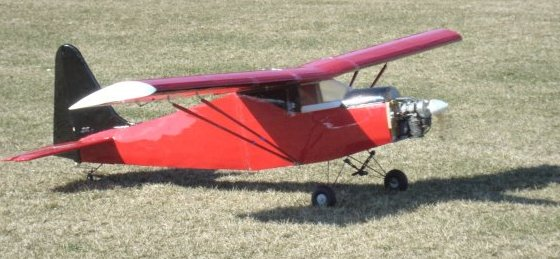
\includegraphics[width=0.5\textwidth]{../images/daedalus.jpg}\\[1cm]
\HRule \\[1cm]
{ \huge \bfseries Rutgers University Autonomous Aircraft Team } \\[0.5cm]
\HRule \\[0.5cm]
{ \large \bfseries Technical Report }
\\[0.5cm]
{ \large \bfseries 2010 AUVSI UAS Competition }
\\[0.5cm]
\HRule \\[1cm]

  {\large Amanda Gaetano, Anthony Garrison, Pat Hickey,}
\\{\large Stephen Indyk, Cogan Noll, John Palmer,}
\\{\large Adrien Perkins, Gregory Quinn, and Michael Varga}
\\[1cm]
\emph{Thank you to our sponsors}
\\ Rutgers University Engineering Governance Council
\\ Rutgers Alumni Association
\\ WINLAB
\\ Invensense, Inc.
\\ ST Micro, Inc.

\vfill
{\large \today}

\end{center}
\end{titlepage}


\begin{abstract}
We will write the abstract after the rest of the paper is finished. If we're really close to the page limit, we may be able to omit it.
\end{abstract}

\section{Introduction}

Brief overview of what we accomplished. This should be a very brief chronology of the engineering we've done to date.

\section{Systems Engineering}

We need to give an overview of our airframe, autopilot, and payload requirments. Amanda or Anthony should decide how to proceed here based on other good papers.

One thing we need is a good justification for having built two fucking giant airframes. Lets point out that we initially assumed a much heavier payload, but found lighter and smaller alternatives as the year went on. We decided it was better to be too big than too small. A large plane with lower wing loading would be easier to control, and easier to recover in case power is lost. (someone check that math)

\section{Flight Vehicle}

At the time of this writing, we have completed and flown a single flight vehicle, which we have named the \emph{Daedalus}.
We have also nearly completed a very similar backup airframe which serve as a backup in case the \emph{Daedalus} has a disaster. The \emph{Knight Two} will be fitted with 

\subsection{Airframe}

We elected to persue a kit-type airplane rather than our own design. 
Our own custom design, the \emph{Icarus}, suffered a catastrophic structural failure last year. From this, we learned that custom structures require much more testing and revision than a proven kit. We also reconsidered our payload requirments and decided we could easily modify a kit plane to accept our autopilot and imaging system.

\subsubsection{Daedalus}

A member of our local R/C club, Tri-County RC \cite{tricountyRC}, donated a ten-foot wingspan high wing trainer to our club. The plane, first built out of foam and balsa from long-lost plans in 1986, was accepted graciously, but required quite a bit of work before it was once again flightworthy. We removed the covering to find water damage and rot which resulted from years of storage. We stripped and rebuilt nearly the entire airframe, adding carbon-fiber reinforcements to the wing in anticipation of increased wing loading due to our payload.

Once rebuilt and covered, we tested the \emph{Daedalus} in our shop to ensure the rebuilt structure was strong enough. Amanda and Anthony, please continue working on this paragraph, describing our testing procedures

Figure goes here: Photos of Daedalus in construction, sandbag testing

Someone please detail the outer dimensions. The inner dimensions, space used for flight electronics, space used for payload underneath. Landing gear height. Number of servos and their locations

Figure may go here: Line drawing of Daedalus. JOHN

\subsubsection{Knight Two}

In order to mitigate a disaster such as we had last year, we decided to build another airframe which could replace the \emph{Daedalus} at short notice. We selected an Aero-Design 12 Foot Telemaster \cite{aerodesign} because it was available as a balsa kit and similar in size to the \emph{Daedalus}.

We named it the \emph{Knight Two} after the Rutgers University mascot, the Scarlet Knight. We may rename it if someone can think of a better name. Pat needed to think up a decent name real fast in order to make this rough draft.

Since our testing plan for the \emph{Daedalus} was successful, we will follow the same plan when, in the coming weeks, we finish building \emph{Knight Two}.

Figure goes here: Photos of Knight Two in construction, sandbag testing

Someone please detail the outer dimensions. The inner dimensions, space used for flight electronics, space used for payload underneath. Landing gear height. Number of servos and their locations

Figure may go here: Line drawing of Knight Two. JOHN

\subsection{Power}

\subsubsection{Engine}

Each airframe has a 45cc gasoline engine. Each airframe has a xx ounce gasoline tank. Based on our flight tests, with climbs to 400 feet AGL, a full xx ounce gasoline tank gives us xx minutes of flight time. (can someone guestimate this? Do we have data from break-in, etc)

\subsubsection{Batteries}

Each airframe has nearly identical flight electronics. To power a Futaba 2.4GHz receiver and 6 servos for a XX minute flight, we selected a 2 cell XX amp hour Lithium Ion battery with a 5v, 10A capacity switching regulator made by Castle Creations. Pat will add more here if he has to.

\section{Autopilot}
Our entry uses an autopilot system based off the open source 
Paparazzi project\cite{paparazziweb}. 
We ported the airborne code to Linux in order to use a single computer for all of our flight hardware and software.

\subsection{Requirments}

We needed to interface with the following hardware components:
\begin{itemize}
	\item GPS
	\item servos
	\item camera
	\item etc.
\end{itemize}

Interfacing with such a large array of devices meant we had to use a ...

\subsection{Hardware}
Single board computer: beagleboard.

Description of each input, output interface.

Figure goes here: Hardware connection diagram. PAT
\subsection{Software}
PAT

Figure goes here: interprocess communication. PAT
\subsection{Ground Station}
Because we based our autopilot software on the Paparazzi project, we were able to make use of their excellent ground control software (GCS) with essentially no modifications.

Detail the capabilities of the Paparazzi GCS.

Figure goes here: Paparazzi ground station screenshot, or whatever. 
\subsection{Tuning and Testing}
PAT

\section{Imaging System}
COGAN, MICHAEL write an overview

\subsection{Camera}

MICHAEL : physical specification of camera (size, 5 megapixel stills). We selected it because...

MICHAEL: camera interfaces: serial and USB 

The camera will be mounted in a pan and tilt unit, which will ... STEVE, PAT

\subsection{Image Processing}
MICHAEL, describe flow of control and images in the camera software.

COGAN, describe computer vision algorithms, and anything else we do

\subsection{Ground Station Interface}

COGAN, describe the ground station interface

Figure goes here: COGAN, provide a screen shot of the ground station in 'action.' We should try to use images that at least look like they were taken of targets from above. Maybe take pictures from 7th floor CORE, like we said we were going to use to train the cv algorithms.

\section{Operation Safety}

PAT

\subsection{Safety Features}

PAT

\subsection{Procedures}

PAT (well i dont know what to do here yet)

\bibliographystyle{plain}
\bibliography{paper}

\end{document}
